Simulating the behavior of an astrophysical system with a fine-granularity is computationally expensive. However, a technique known as \textbf{superresolution} may be able to reduce the cost by simulating the system at a coarse-granularity `big picture' and using some other method to reconstruct the fine-grain `details.' One could use superresolution to refine the resolution in space, time, or both, but the spatial problem is better studied, and I believe more useful for astrophysical simulations.\footnote{Please correct me if I am wrong.}

Spatial superresolution was originally studied for videos. The hidden variable is the function from 2D-position to colors in the camera's perspective. Although it exists continuously, it is only sampled/observed discretely at pixel points.
Any movement between the subject and the observer in subsequent frames shifts the pixel grid slightly to yield a new sampling at \textit{different} gridpoints, as in \cref{classical-superresolution}.
%Features which may have fallen in between pixels in one frame may fall right on a pixel in another frame (because the camera or the subject moved slightly), so the feature's existence in the first frame can be inferred.
This is the `information theoretical' basis for video superresolution given by Katsaggelos et al. \cite{synthesis-lecture}.

\begin{figure}
  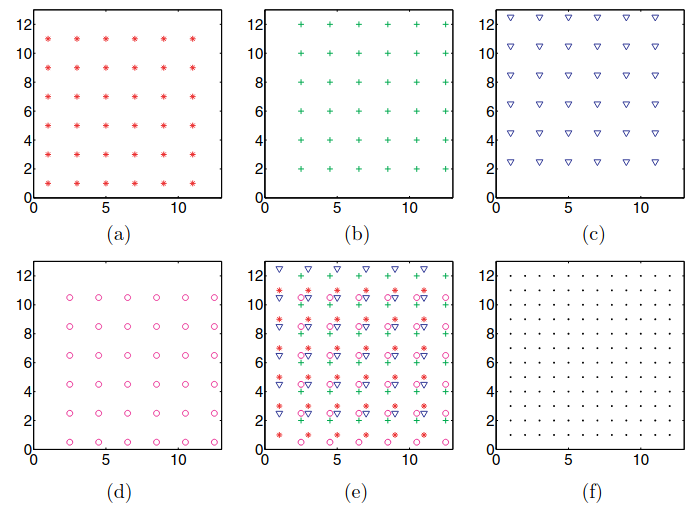
\includegraphics[width=4.5in]{classical-superresolution.png}
  \caption{Low-resolution images (a), (b), (c), and (d), when overlayed, sample the underlying phenomenon at the points in (e). This set of low-resolution images can synthesize a higher-resolution image, (f), with classical superresolution.}
  \label{classical-superresolution}
\end{figure}

However, in superresolution for simulations, the hidden variable is the high-granularity simulation, and it only exists discretely. There are no features in the high-granularity simulation to recover finer than the fine-grain gridpoints. I am not sure this same theoretical justification applies, but perhaps another does: given the ergodic principle, every patch of space should have some patch in the training set that looks similar. In theory, superresolution can work by saving computational resources by learning what happens to small patches of space in the \textbf{training phase} and interpolating a novel patch based in the \textbf{prediction phase}. While neural networks are universal function approximators, a neural network can be more computationally expensive than the function it was trained to approximate (in this case, the fine-grained fluid dynamic simulation), which is what I want to test. Liu et al. \cite{survey} give a survey of deep-learning-based spatial superresolution algorithms for videos. I want to pick one and adapt it for astrophysical systems.
%
%Liu \cite{survey} gives a taxonomy of deep learning superresolution methods. There are some methods which try to learn an alignment between frames. I do not expect these to fair well because they explicitly depend on the information theoretical conditions that may not exist in the fluid simulation case. Therefore, I will select `methods without alignment' and try adapting those codes for astrophysical simulations. \todo{Explain the methods more}

FLASH \cite{FLASH} has been used to simulate supernovae \cite{supernova-simulation}, which I will use as a case study. I will run FLASH many times with randomized inputs at a high-resolution. I will split that data into training data and testing data. Then I will use the former to train a neural network and the later to evaluate it. I will evaluate the mean-squared error, peak signal-to-noise ratio, and Kullback-Leibler divergence from the superresolution solution, \(\hat{f}(\vb{x})\), to the high-resolution solution, \(f(\vb{x})\):

\[
\begin{array}{rcl}
  \text{MSE}(f, \hat{f}) & = & \iiint_{\Omega} (\hat{f}(\vb{x}) - f(\vb{x})) \dd{V} \\
  \text{PSNR}(f, \hat{f}) & = & 20 \log_{10} \frac{\max\limits_\Omega f}{\sqrt{\text{MSE}(f, \hat{f})}} \\
  D_\text{KL}(f || \hat{f}) & = & \iiint_{\Omega} (f(\vb{x}) \log \frac{f(\vb{x})}{\hat{f}(\vb{x})}) dV \\
\end{array}
\]

I hypothesize that for a fixed set of computational resources, the ratio of information gained about the system (KL divergence) per unit of time spent computing will be constant between superresolution and high-resolution simulation, but perhaps superresolution can maintain a PSNR competetive with high-resolution, equivalent to finding an `compression' of the high-resolution data, an information theory sense. So long as the data is not truly random, we know \textit{some} compression must exist, but we do not necessarily know how to find it. A high-information content in a high-granularity may not be necessary, and superresolution is just a method for gaining an intermediate amount of information in a high-granularity.
